\documentclass[10pt]{article}
\usepackage[english]{babel}
\usepackage[latin1]{inputenc}
\usepackage{subfigure}
\usepackage{epsfig}
\usepackage{amsmath}
\usepackage{psfrag}
\parindent 0mm
\textwidth 16cm
\textheight 23cm
\oddsidemargin 0cm
\evensidemargin 0cm
\topmargin -10mm
\newcommand{\vect}[1]{{\bf{#1}}}
\newcommand{\svect}[1]{\boldsymbol{#1}}
\newcommand{\matr}[1]{\boldsymbol{#1}}
\newcommand{\vw}{{\bf{w}}}
\newcommand{\ve}{{\bf{e}}}
\newcommand{\vx}{{\bf{x}}}

\begin{document}
\pagestyle{empty}
\begin{Large}
\begin{bf} 
T-61.5130 Machine Learning and Neural Networks\\ 
\end{bf}
\end{Large}
Karhunen, Hao Tele\\  
\\
\begin{large}
\begin{bf}
Exercise 2,  10.11.2011\\Model answers
\end{bf}
\end{large}
\begin{enumerate}

\item Let the error function be
\begin{equation*}
{\cal E}(\mathbf{w})=w_1^2+10w_2^2,
\end{equation*}
where $w_1$ and $w_2$ are the components of the two-dimensional
parameter vector $\mathbf{w}$. Find the minimum value of ${\cal
E}(\mathbf{w})$ by applying the steepest descent method. Use
$\mathbf{w}(0)=[1,1]^T$ as an initial value for the parameter vector
and the following constant values for the learning rate:
\begin{enumerate} \item $\alpha=0.04$ \item $\alpha=0.1$ \item
$\alpha=0.2$
\item What is the condition for the convergence of this method?
\end{enumerate}

-----------------------------------------------------------

The error function is
\begin{equation*}
{\cal E}(\vw)=w_1^2+10w_2^2,
\end{equation*}
where $w_1$ and $w_2$ are the components of the two-dimensional
parameter vector $\vw$. 

The gradient is
\begin{equation*}
  \nabla_{\vw} {\cal E} (\vw) = \begin{pmatrix} \frac{\partial {\cal E}
      (\vw)}{\partial w_1} \\  \frac{\partial  {\cal E} (\vw) }{\partial
      w_2}\end{pmatrix} = \begin{pmatrix} 2 w_1 \\  20 w_2 \end{pmatrix}.
\end{equation*}

The steepest descent method has a learning rule:
\begin{equation*}
  \begin{split}
    \vw(n+1) & = \vw(n)- \alpha \nabla_{\vw(n)} {\cal E} (\vw(n)) \\
    & = \begin{pmatrix} w_1 \\  w_2 \end{pmatrix} - \alpha
    \begin{pmatrix} 2 w_1 \\  20 w_2 \end{pmatrix} = \begin{pmatrix}
      (1 - 2 \alpha) w_1 \\  (1 - 20 \alpha) w_2 \end{pmatrix} .
  \end{split}
\end{equation*}

It was given $\vw(0) = \begin{pmatrix} 1 & 1 \end{pmatrix}^T$:
\begin{equation*}
    \vw(n+1) = \begin{pmatrix} (1 - 2 \alpha)^{n+1} w_1(0) \\  (1 - 20
      \alpha)^{n+1} w_2(0) \end{pmatrix} = \begin{pmatrix} (1 - 2
      \alpha)^{n+1} \\  (1 - 20 \alpha)^{n+1} \end{pmatrix}. 
\end{equation*}

\begin{enumerate}
\item $\alpha = 0.04$: 
\begin{equation*}
  \vw(n+1) = \begin{pmatrix} 0.92^{n+1} \\
    0.20^{n+1} \end{pmatrix} \xrightarrow[n\rightarrow\infty]{}\begin{pmatrix}0\\0\end{pmatrix}
\end{equation*}

\item $\alpha = 0.1$: 
\begin{equation*}
  \vw(n+1) = \begin{pmatrix} 0.8^{n+1} \\
    (-1)^{n+1} \end{pmatrix} \xrightarrow[n\rightarrow\infty]{}\left\{\begin{array}{cl}\begin{pmatrix}0\\-1\end{pmatrix} & \mbox{,when } n\mbox{ is even}\\
\begin{pmatrix}0\\1\end{pmatrix} & \mbox{,when } n\mbox{ is odd}\end{array}\right.
\end{equation*}

\item $\alpha = 0.2$: 
\begin{equation*}
  \vw(n+1) = \begin{pmatrix} 0.6^{n+1} \\
    (-3)^{n+1} \end{pmatrix} \xrightarrow[n\rightarrow\infty]{}\left\{\begin{array}{cl}\begin{pmatrix}0\\-\infty\end{pmatrix} & \mbox{,when } n\mbox{ is even}\\
\begin{pmatrix}0\\\infty\end{pmatrix} & \mbox{,when } n\mbox{ is odd}\end{array}\right.
\end{equation*}

\item Iteration converges if $| 1 - 2 \alpha | < 1$ and $| 1 - 20 \alpha | < 1 \Rightarrow 0 < \alpha < 0.1$. 
No oscillations occur if $0 < 1 - 2 \alpha < 1$ and $0 < 1 - 20 \alpha < 1 \Rightarrow 0 < \alpha < 0.05$.

\end{enumerate}

\vspace{12mm}

\item The normalized LMS algorithm is described by the following
recursion for the weight vector:
\begin{equation*}
\Hat{\mathbf{w}}(n+1)= \Hat{\mathbf{w}}(n) +\frac{\eta e(n)
\mathbf{x}(n)} {\| \mathbf{x}(n) \|^2},
\end{equation*}
where $\eta$ is a positive constant and $\|\mathbf{x}(n) \|$ is the
Euclidean norm of the input vector $\mathbf{x}(n)$. The error
signal $e(n)$ is defined by
\begin{equation*}
e(n)=d(n)-{\Hat{\mathbf{w}}(n)}^T \mathbf{x}(n),
\end{equation*}
where $d(n)$ is the desired response. For the normalized LMS algorithm to
be convergent in the mean square, show that $0< \eta <2$.

-----------------------------------------------------------

%Iteration converges if $|1-2\alpha|<1$ and $|1-20\alpha|<1
%\Rightarrow 0<\alpha<0.1$. No oscillations occur if $0<1-2\alpha<1$
%and $0<1-20\alpha<1 \Rightarrow 0<\alpha<0.05$
%%\end{enumerate} 

Convergence in the mean square means that
$E\left[e^2(n)\right]\xrightarrow[n\rightarrow\infty]{}\mbox{constant}$.

In the conventional LMS algorithm we have
\begin{equation*}
\vw(n+1)=\vw(n)+\eta e(n)\vx(n)
\end{equation*}
which is convergent in the mean
square if 
\begin{equation*}
0<\eta<\frac{2}{\mbox{sum of mean-square values of the
inputs}}\end{equation*}
or 
\begin{equation*}
0<\eta<\frac{2}{\|\vx(n)\|^2} \forall n.
\end{equation*}
 (This is a stricter condition than the first one!)



In the normalized LMS algorithm we have
\begin{equation*}
\vw(n+1)=\vw(n)+\tilde{\eta}\frac{e(n)\vx(n)}{\|\vx(n)\|^2}
\end{equation*}
Comparing this to the conventional LMS algorithm we have:
\begin{equation*}
\tilde{\eta}=\eta\|\vx(n)\|^2
\end{equation*}

Using this result in the convergence condition yields the condition
for convergence of the normalized LMS algorithm in the mean square as
$0<\tilde{\eta}<2$.

\vspace{2mm}


\vspace{12mm}

\item A linear classifier separates $n$-dimensional
space into two classes using a $(n-1)$-dimensional hyperplane. Points
are classified into two classes, $\omega_1$ or $\omega_2$, depending on
which side of the hyperplane they are located.
\begin{enumerate} \item Construct a linear classifier which is able to
separate the following two-dimensional samples correctly:\\
\begin{align}
&\omega_1: \text{\;} \{[2,1]^T\}, \notag \\
&\omega_2: \text{\;} \{[0,1]^T, [-1,1]^T \}. \notag
\end{align}
\item Is it possible to construct a linear classifier which is able to
separate the following samples correctly? \\
\begin{align}
&\omega_1:\text{\;} \{ [1,1]^T, [2,2]^T \}, \notag \\
&\omega_2: \text{\;} \{ [1,2]^T,[2,1]^T \} \notag
\end{align}
Justify your answer.
\end{enumerate}

-----------------------------------------------------------


\begin{enumerate} 
\item

The separating plane can be expressed as $x_1 = x_2$. This leads to
the separation rule $\vect{w}^T \vect{x}=0$, where $\vect{w}=[-1,1]$.
 
\begin{align}
&\omega_1: \text{\;} \{[2,1]^T\}, \notag \\
&\omega_2: \text{\;} \{[0,1]^T, [-1,1]^T \}. \notag
\end{align}
\psfrag{x1}{$x_1$}
\psfrag{x2}{$x_2$}
\psfrag{w1}{$\omega_1$}
\psfrag{w2}{$\omega_2$}
\begin{center}
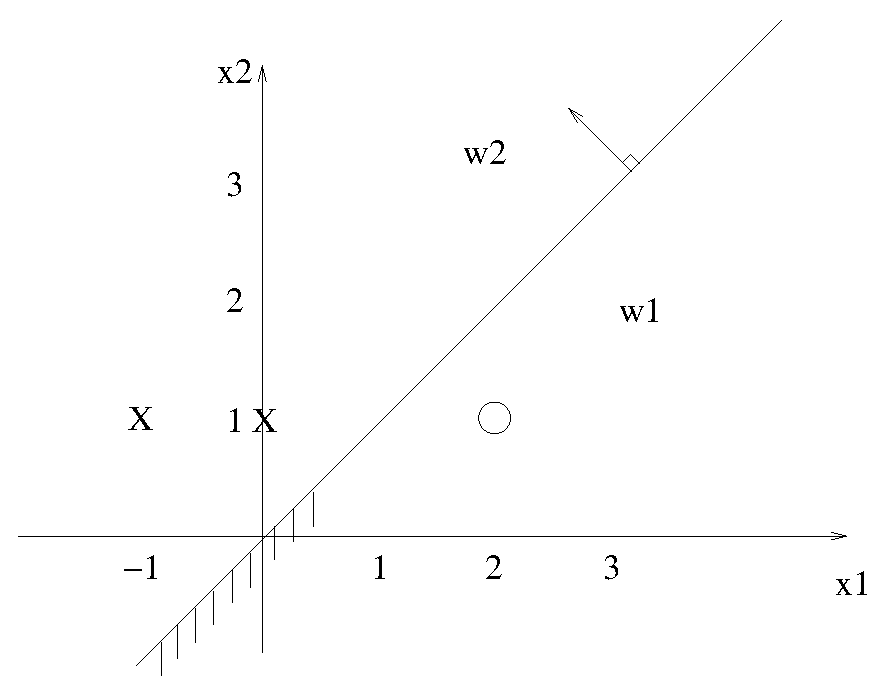
\includegraphics[scale=0.35]{e4_5.eps}
\end{center}

Classifications are carried out as follows:
\begin{equation*}
\left\{\begin{array}{l}
\vw^T\vx<0 \Rightarrow \vx \in \omega_1\\
\vw^T\vx\geq 0 \Rightarrow \vx \in \omega_2\\
\end{array}\right.
\end{equation*}

\item

\begin{align}
&\omega_1:\text{\;} \{ [1,1]^T, [2,2]^T \}, \notag \\
&\omega_2: \text{\;} \{ [1,2]^T,[2,1]^T \} \notag
\end{align}
\begin{center}
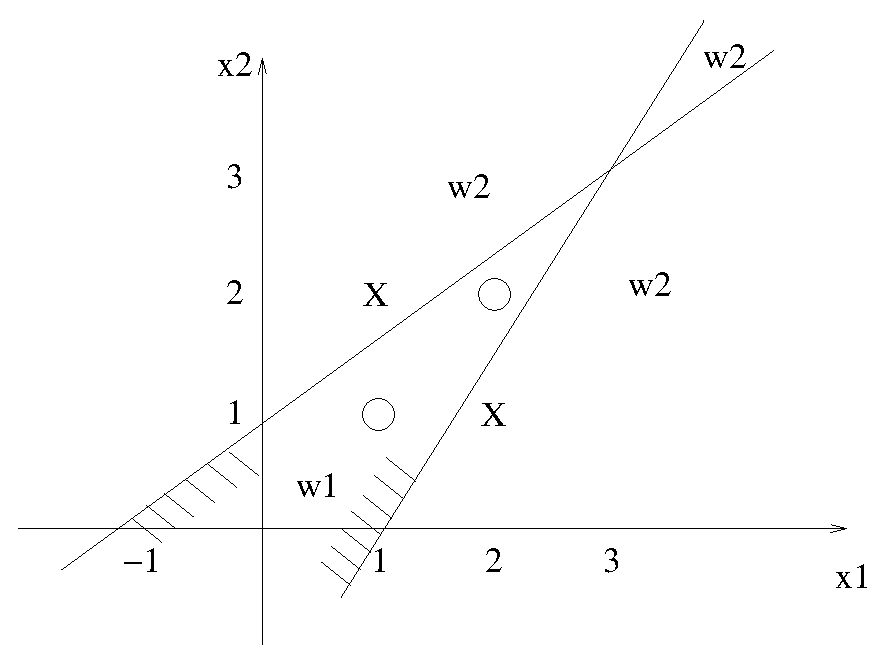
\includegraphics[scale=0.35]{e4_5b.eps}
\end{center}

It is not possible to separate the classes with a single
hyperplane. At least two hyperplanes are required to separated the
classes correctly.

\end{enumerate}

\vspace{12mm}

\item (Hamm \& Kostanic: 2.8) Write a computer program using a perceptron (see Figure 2.30) to classify
the digits given in Figure 2.41. The number of neurons in the output layer should be equal to the
number of digits.

-----------------------------------------------------------

In Section 2.6.2 we derived the perceptron learning rule for the case of a network with a single
output. For this problem we derive a more general learning rule that can be used to train a single layer
perceptron neural network with multiple outputs.

The output of the network to the qth training pattern is given by

\[
\hat{\vect{y}}_q = f(\matr{W}\vect{x}_q)
\]

where $\matr{W}$ is the weight matrix, $\vect{x}q$ is the $q$:th input pattern, $\vect{y}_q$ is
the $q$:th target output pattern and $f(\cdot)$ is the nonlinear activation
function.

For every training input-output pair an error vector can be formed as:

\[
\vect{e}_q = \hat{\vect{y}}_q - \vect{y}_q
\]

Similar to the case of the single-output perceptron network, the
objective of the training process is to minimize the expected value of
the square of the error vector norm. In other words, the optimization
criterion is given as

\[
J(\matr{W}) = \frac{1}{2}E \lbrace \vect{e}_q^T\vect{e}_q \rbrace
\]

Adopting the same approach presented in Section 2.6.2, we use the instantaneous estimate of the error
surface to derive a learning rule of the form

\[
\matr{W}(k+1) = \matr{W}(k) - \mu \frac{\partial J(\matr{W})}{\partial \matr{W}} \approx 
\matr{W}(k) -
\frac{1}{2} \mu
\frac{\partial}{\partial \matr{W}} [\vect{e}_q^T\vect{e}_q]
\]

where $\mu>0$, is the learning rate parameter. This approximation
gives the following update formula for the weights

\[
\matr{W}(k+1) = \matr{W}(k) - \mu \vect{x}_q \vect{e}_q^T {\text
  diag}
\lbrace f(\vect{w}_1^T\vect{x}q) \hspace{2mm}...\hspace{2mm} f(\vect{w}_m^T\vect{x}_q) \rbrace
\]

In the special case when the activation function has a form

\[
f(v) = \tanh(\alpha v)
\]

we have

\[
f'(v) = \alpha [1 - f^2(\alpha v)]
\]

and the weight update equation becomes

\[
\matr{W}(k+1) = \matr{W}(k) - \mu \alpha \vect{x}_q \vect{e}_q^T {\text diag} \lbrace 1-\hat{\vect{y}}_{q1}^2
 \hspace{2mm}...\hspace{2mm} 1-\hat{\vect{y}}_{qm}^2 \rbrace
\]

In Matlab this learning rule can be implemented as follows:

\begin{small}
\begin{verbatim}
function [W,E] = percep(P,T,Tp)

% PERCEPT implements perceptron NN
%
% Synopsis
%
%	[W,E] = percep(P,T,Tp)
%
% 	where:
% 	P			- 	RxQ matrix of Q input vectors
%	T			- 	1xQ matrix of target values
%	Tp			- 	training parameters
%	Tp(1)		- 	learning rate parameter (Default 0.001)
%	Tp(2)		- 	time constant for learning rate perimeter (see (2.36))
%				- 	if set to zero the learning rate is  constant (Default 0)
%		Tp(3) - 	maximum number of iterations (Default 1000)
%		Tp(4) - 	mean square error goal (Default 0)
%		Tp(5)	- 	slope of the activation function sigmoid
%	W			- 	weights 
%  E			- 	error trajectory

% Set the defaults

if nargin == 2
   Tp = [0.001 0 1000 0 1];
end

% Initialize weights

[N,Q] = size(P);
[M,Q] = size(T);

W = 0.001 * randn(N,M);

% Network training

iter = 0;
E = [];

while iter < Tp(3)
   iter = iter + 1;
   Y = 0;
   for k = 1:Q
      if Tp(2) ~= 0
         yout = tanh(Tp(5)*W'*P(:,k));
         Y = Y+1/Q*norm((yout-T(:,k)))^2;
         W = W-Tp(1)/(1+k/Tp(2))*P(:,k)*(yout-T(:,k))'*diag(1-yout.^2);
      else 
         yout = tanh(Tp(5)*W'*P(:,k));
			Y = Y+1/Q*norm((yout-T(:,k)))^2;
         W = W-Tp(1)*P(:,k)*(yout-T(:,k))'*diag(1-yout.^2);
      end
   end
   E = [E Y];
   if Y < Tp(4) break;
   end
end

\end{verbatim}
\end{small}

\end{enumerate}

\vspace{12mm}

5. 
\begin{align*}
J(\vw)&=\frac{1}{2}E[e^2(n)]=\frac{1}{2}E[(d(n)-\mathbf{x}(n)^T\vw)^2] \\
&=
\frac{1}{2} E[d(n)^2] - \vw^T E[ d(n) \mathbf{x}(n)  ]  + 
\frac{1}{2} \vw^T E[\textbf{x}(n) \textbf{x}(n)^T ] \vw \mbox{.}
\end{align*}
%
Now if we define 
\begin{equation*}
\textbf{C}_x = E[\textbf{x}(n) \textbf{x}(n)^T ]
\end{equation*}
and
\begin{equation*}
\textbf{p} = E[d(n) \textbf{x}(n) ] \mbox{,}
\end{equation*}
then
\begin{align*}
J(\vw) = \frac{1}{2} E[d(n)^2] - \vw^T \textbf{p}  + 
\frac{1}{2} \vw^T \textbf{C}_x \vw \mbox{.}
\end{align*}
%
The gradient of this is
\begin{align*}
\nabla J =   \textbf{C}_x \vw - \textbf{p} \mbox{.}
\end{align*}
%
Now setting this to zero, we can solve for the minimizer of $J$:
\begin{equation*}
\textbf{w}^* = \textbf{C}_x^{-1} \textbf{p} \mbox{.}
\end{equation*}
Now 5(a) is solved by substituting $\textbf{w}^*$ into the expression for $J$.
5(b) follows by a straightforward calculation or alternatively, we may observe
that $\nabla_{\textbf{w}^*} J = 0$ and the Hessian of $J$ at $\textbf{w}^*$ is $\textbf{C}_x$.
The higher order derivatives are zero, because $J$ is a second order polynomial with respect
to $\textbf{w}$ and thus
\begin{equation*}
J(\vw) = J( \textbf{w}^* ) + \frac{1}{2} ( \vw - \textbf{w}^* ) \textbf{C}_x ( \vw - \textbf{w}^* ) \mbox{.}
\end{equation*}


\end{document}             % End of document.
